\documentclass[10, sigconf]{acmart}

\usepackage{graphicx,xspace,verbatim,comment}
\usepackage{hyperref,array,color,balance,multirow}
\usepackage{balance,float,url,amsfonts,alltt}
\usepackage{mathtools,rotating,amsmath,amssymb}
\usepackage{color,ifpdf,fancyvrb}
\usepackage{etoolbox,listings,subcaption}
\usepackage{bigstrut,morefloats,pbox}
\usepackage{amsmath}
\usepackage{algorithm}
\usepackage[noend]{algpseudocode}
\usepackage{booktabs}

\newtheorem{theorem}{Theorem}[section]
\newtheorem{proposition}{Proposition}[section]
\newtheorem{corollary}[theorem]{Corollary}
\newtheorem{lemma}[theorem]{Lemma}
\newtheorem{definition}{Definition}[section]
\newcommand{\eat}[1]{}
\newcommand{\red}{\textcolor{red}}
\newcommand{\system}{\textsc{Krypton}}

\makeatletter
\def\BState{\State\hskip-\ALG@thistlm}
\makeatother 

\newenvironment{packeditems}{
\begin{itemize}
  \setlength{\itemsep}{1pt}
  \setlength{\parskip}{0pt}
  \setlength{\parsep}{0pt}
}{\end{itemize}}

\newenvironment{packedenums}{
\begin{enumerate}
  \setlength{\itemsep}{1pt}
  \setlength{\parskip}{0pt}
  \setlength{\parsep}{0pt}
}{\end{enumerate}}


\newcolumntype{P}[1]{>{\centering\arraybackslash}p{#1}}

\DeclareMathOperator*{\argmin}{arg\,min}

\setcopyright{none}
\settopmatter{printacmref=false}
\renewcommand\footnotetextcopyrightpermission[1]{} % removes footnote with 
\pagestyle{plain} % removes running headers

\begin{document}
\title{\textsc{Kryton}: A System for Accelerating Occlusion based Deep CNN Explainability Workloads}

\author{Supun Nakandala \hspace{7mm} Arun Kumar}
\affiliation{%
  \institution{University of California, San Diego}
}
\email{{snakanda, arunkk}@eng.ucsd.edu}


\begin{abstract}
Deep Convolution Neural Networks (CNN) have revolutionized the field of computer vision with even surpassing human level accuracy in some of the image recognition tasks such as ImageNet challenge. Thus they are now being deployed in many real-world use cases using a paradigm called \textit{transfer learning}. However one of the major criticisms pointed against Deep CNNs is the black-box nature of how they make predictions. This is a critical issue when applying CNN based approaches to critical applications such as in health care where the explainability of the predictions is also very important. For interpreting CNN predictions several approaches has been proposed and one of the widely used method in image classification tasks is occlusion experiments. In occlusion experiments one would mask the regions of the input image using a small grey or black patch and record the change in the predicted label probability. By systematically changing the position of the patch location, a sensitivity map can be generated from which the regions in the input image which influence the predicted class label most can be identified. However, this method requires performing multiple forward passes of CNN inference for explaining a single prediction and hence very time consuming.
We present \system, the first data system to elevate occlusion experiments to a declarative level and enable automated \textit{incremental} and \textit{approximate} inference optimizations. Experiments with real-world datasets and deep CNNs show that \system~can enable up to 10x speedups.
\end{abstract}

\maketitle

%!TEX root = <main.tex>
\section{Introduction}
Deep Convolution Neural Networks (CNNs) are now the state of the art method for many image prediction tasks~\cite{imagenet}. Thus, there is growing interest in adopting deep CNNs in various application domains, including healthcare~\cite{kermany2018identifying, islam2017abnormality}, agriculture~\cite{mohanty2016using}, security~\cite{arbabzadah2016identifying}, and sociology~\cite{wang2017deep}. Remarkably, even the US Food and Drug Administration recently approved the use of deep CNNs in radiology to assist radiologists in processing X-rays and other scans, cross-checking their decisions, and even mitigating the shortage of radiologists~\cite{fdaretinopathy,radiologistshortage}.

\begin{figure}[t]
% \vspace{-4mm}
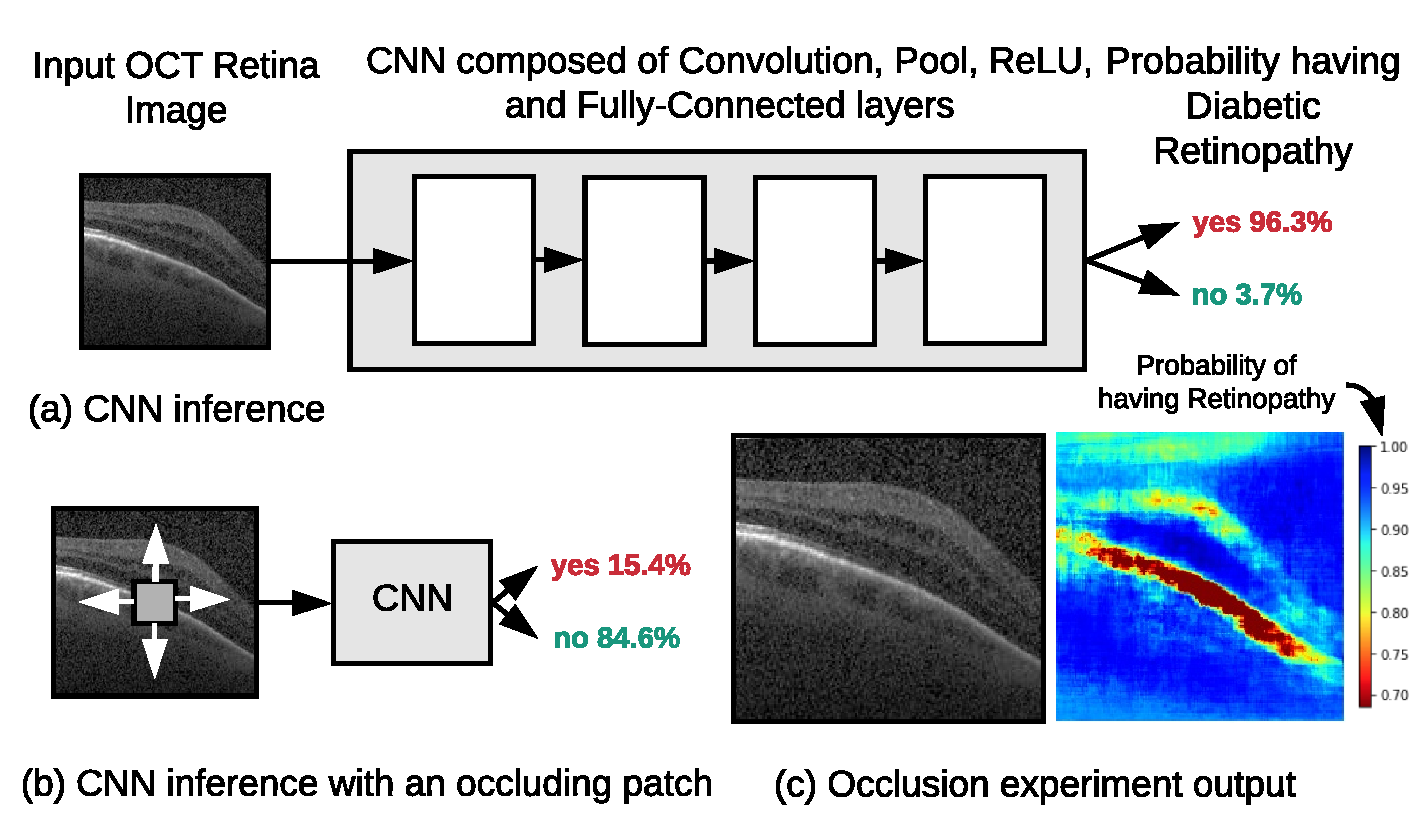
\includegraphics[width=\columnwidth]{./images/krypton_overview}
\caption{(a) Using a CNN to predict diabetic retinopathy in an OCT image/scan. (b) Occluding a part of the image changes the prediction probability. (c) By moving the occluding patch, a sensitivity heat map can be produced.}
\label{fig:krypton_overview}
\vspace{-4mm}
\end{figure}

Despite their successes, a key criticism of CNNs is that their internal workings are unintuitive to non-technical users. Thus, users often seek an ``explanation'' for why a CNN predicted a certain label. Explanations can help users trust CNNs~\cite{ribeiro2016should}, especially in high stakes applications such as radiology~\cite{jung2017deep}, and are a legal requirement for machine learning applications in some countries~\cite{gdpr}. How to explain a CNN prediction is still an active research question, but in the practical literature, an already popular mechanism for CNN explanations is a simple procedure called \textit{occlusion-based explanations}~\cite{zeiler2014visualizing}, or OBE for short.

OBE works as follows. Place a small square patch (usually gray or black) on the image to occlude those pixels. Rerun CNN inference, illustrated in Figure~\ref{fig:krypton_overview} (a), on the occluded image. The probability of the predicted label will change, as Figure~\ref{fig:krypton_overview} (b) shows. Repeat this process by moving the patch across the image to obtain a sensitivity \textit{heat map} of the probability changes, as Figure~\ref{fig:krypton_overview} (c) shows. This heat map will highlight regions of the image that were highly sensitive or ``responsible'' for the prediction (red/orange color regions). Such \textit{localization} of the regions of interest allows users to gain intuition on what ``mattered'' for the CNN prediction. For instance, the heat map can highlight the diseased areas of a tissue image, which a radiologist can then inspect more deeply for further tests. Overall, OBE is popular because it is easy for non-technical users to understand.

Alas, OBE is highly computationally expensive. Deep CNN inference is already expensive; OBE just amplifies it by issuing a large number of CNN re-inference requests (often 1000s)~\cite{ketkar2017introduction}. For example,~\cite{zintgraf2017visualizing} report over 500,000 re-inference requests for OBE on one image, which took 1hr even on a GPU! Such long wait times can hinder users' ability to consume explanations and reduce their productivity. One could use more compute hardware, if available, since OBE is embarrassingly parallel across re-inference requests. But throwing more machines at it may not always be affordable, especially for domain scientists, or feasible in all settings, e.g., in mobile clinical diagnosis. Using extra resources can also raise monetary costs, especially in the cloud.

In this paper, we use a database-inspired lens to formalize, optimize, and accelerate OBE. We start with a simple but crucial observation: \textit{the occluded images are not disjoint but share most of their pixels; so, most of CNN re-inference computations are redundant.} This observation leads us to connect OBE with two classical data management concerns: \textit{incremental view maintenance} (IVM) and \textit{multi-query optimization} (MQO). Instead of treating a CNN as a ``blackbox,'' we open it up and formalize \textit{CNN layers} as ``queries.'' Just like how a relational query coverts relations to other relations, a CNN layer converts \textit{tensors} (multidimensional arrays) to other tensors. So, we reimagine OBE as \textit{a set of tensor transformation queries} with incrementally updated inputs. With this fresh database-inspired view, we introduce several \textit{novel CNN-specific query optimization techniques} to accelerate OBE.

Our first optimization is \textit{incremental CNN inference}. We \textit{materialize} all tensors produced by the CNN's layers on the given image. For every re-inference request in OBE, instead of rerunning CNN inference from scratch, we treat it as an IVM query, with the ``views'' being the tensors. We rewrite such queries to \textit{reuse} as much of the materialized views as possible and recompute only what is needed, thus \textit{avoiding computational redundancy}. Such rewrites are non-trivial because they are closely tied to the complex geometric dataflows of CNN layers. We formalize such dataflows to create an \textit{algebraic framework} of CNN query rewrites. We also create a static analysis routine to predict how much computations can be saved before running any inference. Going further, we batch all re-inference requests in OBE to reuse the \textit{same} materialized views. This is a form of MQO, albeit interwoven with our IVM, leading to a novel \textit{batched incremental CNN inference} procedure. We also create a GPU-optimized kernel for our procedure. To the best of our knowledge, this is the first instance of IVM being fused with MQO in query optimization, at least for CNN inference.

We then introduce two novel \textit{approximate inference} optimizations that allow users to tolerate some degradation in visual quality of the heat maps produced to reduce runtimes further. These optimizations build upon our incremental inference optimization to trade off heat map quality in a user-tunable manner. Our first approximate optimization, \textit{projective field thresholding}, draws upon an idea from neuroscience and exploits the internal semantics of how CNNs work. Our second approximate optimization, \textit{adaptive drill-down}, exploits the semantics of the OBE task and the way users typically consume the heat maps produced. We also present intuitive automated parameter tuning methods to help users adopt these optimizations.

We prototype our ideas in the popular deep learning framework PyTorch to create a tool we call \system. It works on both CPU and GPU and currently supports a few popular deep CNNs (VGG16, ResNet18, and InceptionV3). We perform a comprehensive empirical evaluation of \system ~with three real-world image datasets from recent radiology and computer vision papers. \system ~yields up to $35$X speedups over the current dominant practice of running re-inference with just batching for producing high-quality approximate heat maps and up to $5$X speedups for producing exact heat maps. We then analyze the utility of each of our optimizations. Overall, this paper makes the following contributions:

\vspace{-2.5mm}
\begin{itemize}
	\item To the best of our knowledge, this is the first paper to formalize and optimize the execution of occlusion-based explanations (OBE) of CNN predictions from a data management standpoint.

	\item We cast OBE as an IVM problem to create a novel and comprehensive algebraic framework for incremental CNN inference. We also combine our IVM technique with an MQO-style technique to further reduce computational redundancy in CNN inference.

	\item We present two novel approximate inference optimizations for OBE that exploit the semantics of CNNs and properties of human perception.

	\item We prototype our ideas in a tool, \system, and perform an extensive empirical evaluation with real data and deep CNNs. \system ~speeds up OBE by even over an order of magnitude in some cases.

\end{itemize}

\vspace{-2.5mm}
\noindent \textbf{Outline.} 
Section 2 explains our problem setup, assumptions, formalization of the dataflow of CNNs. Section 3 presents our incremental inference and multi-query optimizations. Section 4 presents our approximate inference optimizations. Section 5 presents the experiments. We discuss other related work in Section 6 and conclude in Section 7.


\section{Background}

\vspace{2mm}
\noindent \textbf{Deep CNNs.} Deep CNNs are a type of neural networks specialized for image data.
They exploit spatial locality of information in image pixels to construct a hierarchy of parametric feature extractors and transformers organized as layers of various types: \textit{convolutions}, which use image
filters from graphics, except with variable filter weights, to extract features; \textit{pooling}, which subsamples features in a spatial
locality-aware way; \textit{batch-normalization}, which normalizes the output of the layer; \textit{non-linearity}, which applies a non-linear transformation (e.g., ReLU); \textit{fully connected}, which is a multi-layer perceptron; and \textit{softmax}, which emits predicted probabilities to each class label.
In most ``deep'' CNN architectures, above layers are simply stacked together with ones output is simply fed as the input to the other, while adding multiple layers element-wise or stacking multiple layers together to produce a new layer is also present in some architectures.
Popular deep CNN model architectures include AlexNet \cite{alexnet}, VGG \cite{vggnet}, Inception~\cite{inception}, ResNet~\cite{resnet}, SqueezeNet~\cite{squeezenet}, and MobileNet~\cite{mobilenets}.

% In this work, the discussion and evaluation is focused on VGG-16 (16 layer version), ResNet-18 (18 layer version) and Inception-V3 (version 3) which are three widely used CNN models in real world transfer learning applications.
% Nevertheless, our work is orthogonal to the specifics of a particular architecture and the proposed approaches can be easily extended to any architecture.

\vspace{2mm}
\noindent \textbf{Deep CNN Explainability} With image classification models, natural question is if the model is truly identifying objects in the image or just using surrounding or other objects for making false prediction.
The various approaches used to explain CNN predictions can be broadly divided into two categories, namely gradient based and perturbation based approaches. Gradient based approaches generate a sensitivity map by computing the partial derivatives of model output with respect to every input pixel via back propagation.
In perturbation based approaches the output of the model is observed by masking out regions in the input image and there by identify the sensitive regions. The most popular perturbation based approach is occlusion experiments which was first introduced by Zeiler et. al. \cite{zeiler2014visualizing}.
Even though gradient approaches require only a single forward inference and a single backpropagation to generate the sensitivity map, the output may not be very intuitive and hard to understand because the salient pixels tend to spread over a very large are of the input image.
Also the back-propagation based methods are based on the AI researchers’ intuition of what constitutes a “good” explanation. But if the focus is on explaining decision to a human observer, then the approach used to produce the explanation should have a structure that humans accept~\cite{miller2017explanation}.
As a result in most real world use cases such as in medical imaging, practitioners tend to use occlusion experiments as the preferred approach for explanations as they produce high quality fine grained sensitivity maps despite being time consuming~\cite{jung2017deep}.

Over the years there has been several modifications proposed to the original occlusion experiment approach. More recently Zintgraf. et. al. \cite{zintgraf2017visualizing} proposed a variation to the original occlusion experiment approach named \textit{Prediction Difference Analysis}. In this method instead of masking with a grey or black patch, samples from surrounding regions in the image are chosen as occlusion patches.
In our work we mainly focus on the original occlusion experiment method. But, the methods and optimizations proposed in our work are readily applicable to more advanced occlusion based explainability approaches.

\section{Preliminaries and Overview}
In this section we formalize the internals of a Deep CNN which will be later used to propose our incremental inference approach in Section 3. We then state the problem studied, explain our assumptions, and given an overview of \system.

\subsection{Deep CNN Internals}
CNNs are composed of a number of different layers: \textbf{convolution} layer, \textbf{pooling} layer (average or max pooling), \textbf{activation} layer, and \textbf{fully-connected} layer.

The main difference of CNNs compared to other neural networks is that they make the explicit assumption that the input is always going to be an image.
This assumption enables them to incorporate several architectural properties into the CNN architecture which reduce the amount of computations required for inference and the amount of learnable parameters.
Neurons in a particular layer of a CNN are organized into 3D volumes with width, hight, and depth dimensions.
For example the images in ImageNet dataset can be treated as an input volume of activations having dimensions of $224\times224\times3$.
Unlike in typical neural networks, a neuron in a convolution layer is only connected to a small region of the layer before it, instead of all the neurons in a full-connected manner.
However this is changed in the last layer (or last few layers) of a CNN in which a neuron is connected to all the neurons in the layer below in a fully connected manner. 

A Deep CNN is composed of several different types of layers. The main types used to build a CNN are: Convolutional Layer, ReLu Layer, Pooling Layer, Fully-Connected Layer and Softmax Layer. Usually Convolution and Fully-Connected are always followed by a ReLu layer which performs a activation wise function which outputs the max of zero of the weighted sum of activations of the connected neurons. Convolution and Pooling layers are stacked alternately to form a cascade of layers and at the end Full-Connected layers are used. A Softmax layer is used at the end of Fully-Connected Layers to output the class probabilities.
Generally in CNNs the activation volumes and filter maps, height and width of the spatial resolution is set to be the same producing square matrices.
Figure. \ref{fig:vgg16} demonstrates how these layers are stacked together to form VGG16 CNN architecture.
Next we will look into Convolutional and Pooling Layers in more detail.

\begin{figure}
  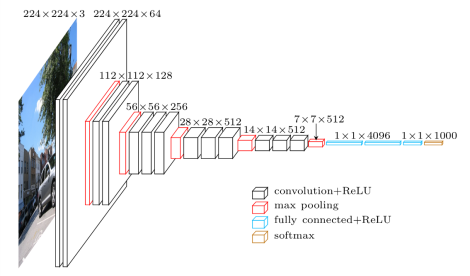
\includegraphics[width=\columnwidth]{./images/vgg16}
  \caption{VGG16 CNN Architecture}
  \label{fig:vgg16}
\end{figure}

\subsubsection{Convolutional Layer}
Convolutional Layer (Conv) is the most important type of layer in a CNN architecture. Also it is the most computationally intensive layer which accounts up to 90\% (or more) of the total computations in a Deep CNN model.
Conv layer parameters consist of set of learnable filters each of which has small spatial dimensions but extends across the depth of the input volume.
For example the first Conv layer of VGG16 model has 64 filter and each has a spatial dimension of $3\times3$ and a depth of $3$ (corresponding to the color depth of the image). In contrast the second Conv layer has 64 filters with the spatial dimension of $3\times3$ but with a depth of $64$ (the depth of the activation volume of layer 1).
A filter is convolved across the height and width dimensions of the input volume producing a 2D feature map where each activation is calculated by the dot product between the filter parameters and the activations of the input volume.
Note that here, only a small portion of the total activations in the input volume, which are spatially collocated together, are used to calculate the activation of an output neuron (see Figure. \ref{fig:conv_local_comp}).
Stacking the 2D feature maps produced for all the filter(e.g VGG16 first Conv layer has 64 filters) a output 3D activation map is created.
At the training time the parameters of the filters are updated using backpropagation and stochastic gradient descent such that these parameters learn to identify different visual concepts (eg. edges, color blotches, and high level objects such human faces) from the activation volume of the layer below \cite{zeiler2014visualizing}.

\begin{figure}
  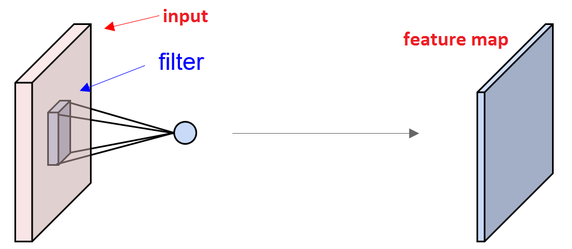
\includegraphics[width=\columnwidth]{./images/cnn_local_computation}
  \caption{Output feature map is computed by performing a dot product between filter values and the input activations}
  \label{fig:conv_local_comp}
\end{figure}

In addition to performing spatial convolutions, Conv layers can optionally reduce the spatial resolution of features volumes. Two hyper-parameters control the size of the output feature volume: the \textbf{stride}, and \textbf{zero-padding}.

\textbf{stride}: When moving the filter across the input volume a stride value has to be specified. When the stride is set to one, the filter is moved one pixel at a time. If the stride is larger than 1, for example setting it to two, the filter is moved 2 pixels at a time producing a smaller output spatial resolution.

\textbf{zero-padding}: Sometimes before performing the filter convolution it is beneficial to pad the input volume with zeros around the border to obtain the required output size. Also, by padding with zeros we can ensure that the input and output volumes will have the same spatial resolution when the stride is set to one.

Given the size of the input volume (\textbf{W}), size of the filter (\textbf{F}), amount of zero-padding (\textbf{P}), and the stride (\textbf{S}) the size of the output volume can be computed by (\textbf{W} - \textbf{F} + 2\textbf{P})/\textbf{S} + 1. For example in VGG16 first Conv layer, the input and output size is $\textbf{W}=224$ and the filter size is set to $\textbf{F}=3$ and is stride is set to $\textbf{S}=1$. To produce the output of same size the padding value should be set to $\textbf{P}=1$. Also note that the potential values for \textbf{W}, \textbf{F}, \textbf{P}, and \textbf{S} has mutual constraints as the output size has to be an integer.

\subsubsection{Pooling Layer}
CNNs architectures periodically insert Pooling Layers to mainly to reduce the spatial resolution of output features maps and also to introduce translational invariance to the image predictions. The pooling layer operated independently on each input feature map along the depth dimension and applies a local filter such as \textbf{max(...)}. The most typical form of Max Pooling is to apply a filter map of size $2\times2$ with a stride of 2 which reduces the height and width of the input feature map by a factor of 2 and discard $75\%$ of the activations. In general when applying a Pooling filter of size \textbf{F} on an input feature volume of size \textbf{W} with a stride of \textbf{S} the produced output volume will have a size of (\textbf{W} - \textbf{F})/\textbf{S} + 1.

\subsection{Computational Cost of Deep CNNs}
Deep CNNs are highly compute intensive and out of the different types of layers, Conv layers contributes to $90\%$ (or more) of the computations. One of the widely used way to estimate the computational cost of a Deep CNN is to estimate the number of fused multiply add (FMA) floating point operations (FLOPs) required for a single forward inference.

Conv layer producing an output feature map of size (\textbf{$W_2$}$\times$\textbf{$W_2$}$\times$\textbf{$D_2$}) from an input feature map of (\textbf{$W_1$}$\times$\textbf{$W_1$}$\times$\textbf{$D_1$}) using a filter of size (\textbf{$F$}$\times$\textbf{$F$}$\times$\textbf{$D_1$}) will require \textbf{$F$}$\times$\textbf{$F$}$\times$\textbf{$D_1$}$\times$\textbf{$W_2$}$\times$\textbf{$W_2$}$\times$\textbf{$D_2$} FMA operations.
For example in VGG16, computing a single activation of the first Conv volume requires 27 $(3\times3\times3)$ FMA operations and computing the whole output Conv volume requires 84 $(3\times3\times3\times224\times224\times64)$ Mega FMA operations. A Fully-Connected Layer reading \textbf{$N_1$} input activations and producing \textbf{$N_2$} output activations requires \textbf{$WN1$}$\times$\textbf{$N_2$} FMA operations.
For example, the first Fully-Connected Layer in VGG16 model requires 98 ($(7\times7\times512)\times4096$) Mega FMA operations.
The floating points operations performed by other layers (e.g. ReLu and Pooling) are relatively very smaller than that performed by Conv and Full-Connected Layers and hence neglected in compute cost analyses.

Alternatively one could also evaluate the computational cost of a CNN model by actually performing a CNN inference and recording the wall clock time. For making CNN inference (and in generally for deep neural networks) one could use either CPUs or GPUs. GPUs are generally an order of magnitude faster than CPUs. However the overhead of data transfer to the GPUs is higher than that of CPUs. Hence by batching multiple input images the overhead can be amortized. Figure \ref{fig:compute_cost} shows the theoretically floating point operations required and actual per image inference time on CPU and GPU for several widely used Deep CNN models (AlexNet, VGG16, ResNet50, and MobileNet).

\begin{figure}
  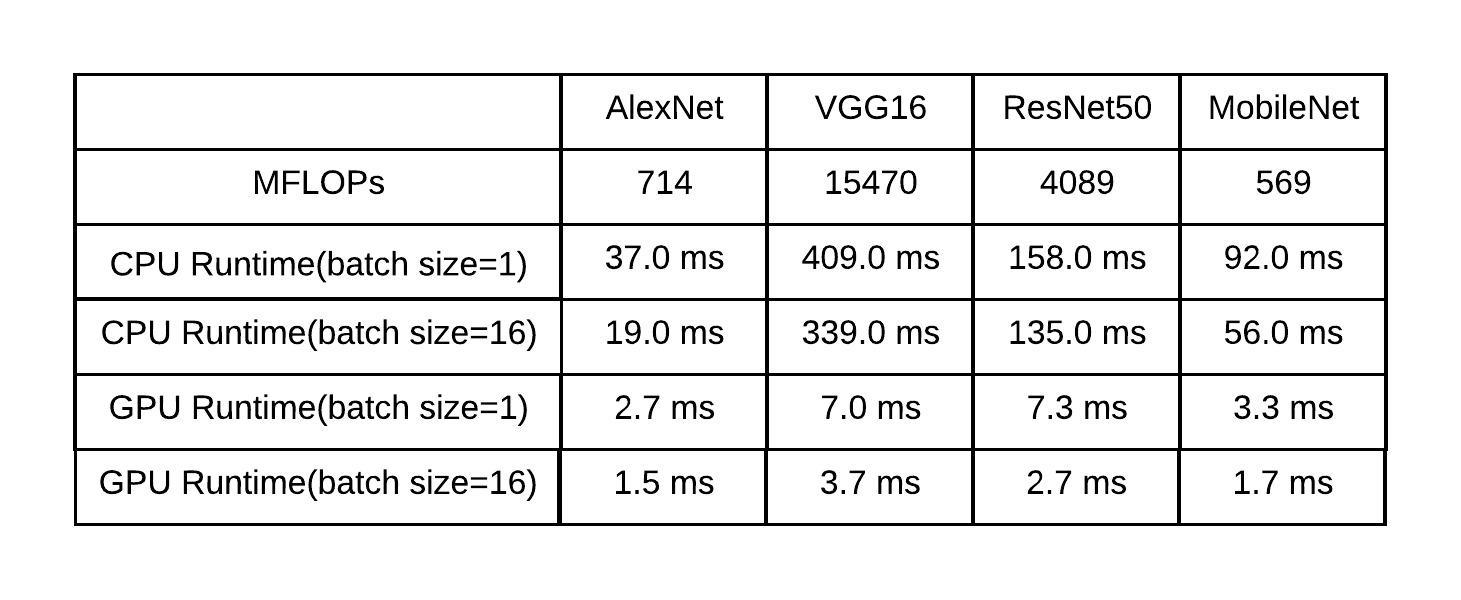
\includegraphics[width=\columnwidth]{./images/compute_cost}
  \caption{Compute cost of widely used Deep CNNs. (CPU: Intel(R) Core(TM) i7-6700 CPU \@ 3.40GHz machine with 32 GB Ram, GPU: Nvidia Titan Xp, Deep Learning Library: PyTorch 0.3.1)}
  \label{fig:compute_cost}
\end{figure}


\section{Optimizations}

\subsection{Incremental Inference of Convolution and Pooling Layers}\label{sec:ivm}

As explained earlier, occlusion experiments are performed by performing CNN inference on large amounts of images which are generated by masking a small square region of the input image.
When we compare the original image and a single masked image most of the pixel values are not changed. For example for an input image of size $224\times224$ pixels when using a occlusion patch of size $16\times16$ only $0.5\%$ of the pixels are different between the two images.
As a result of this performing a full convolution inference on the masked image introduces lot of redundant computations which could potentially be saved.
For example consider the simple 2D convolution example shown in Figure. \ref{fig:perturbation}.
The input feature map is square map with size $W_1=4$ and is convolved by a 2D square filter kernel of size $F=3$ with a stride of $S=1$ to produce an output feature map of size $W_2=4$.
The input feature map is also padded with zeros with a pad width of $P=1$ to ensure that both the input feature map size and the output feature map size is the same (this step is optional).
Now if we update the top left corner value in the input feature map (marked in red), it will only update 4 output values at the top left corner of the output feature map which corresponds to filter map positions on the input feature map with some overlapping with the updated input value.
Even though in this example the amount of updated values in the output feature maps is $25\%$ of the total output values, in general with larger feature map sizes the portion of updated values will be much smaller.
This analysis similarly applies to pooling layers.

\begin{figure}
  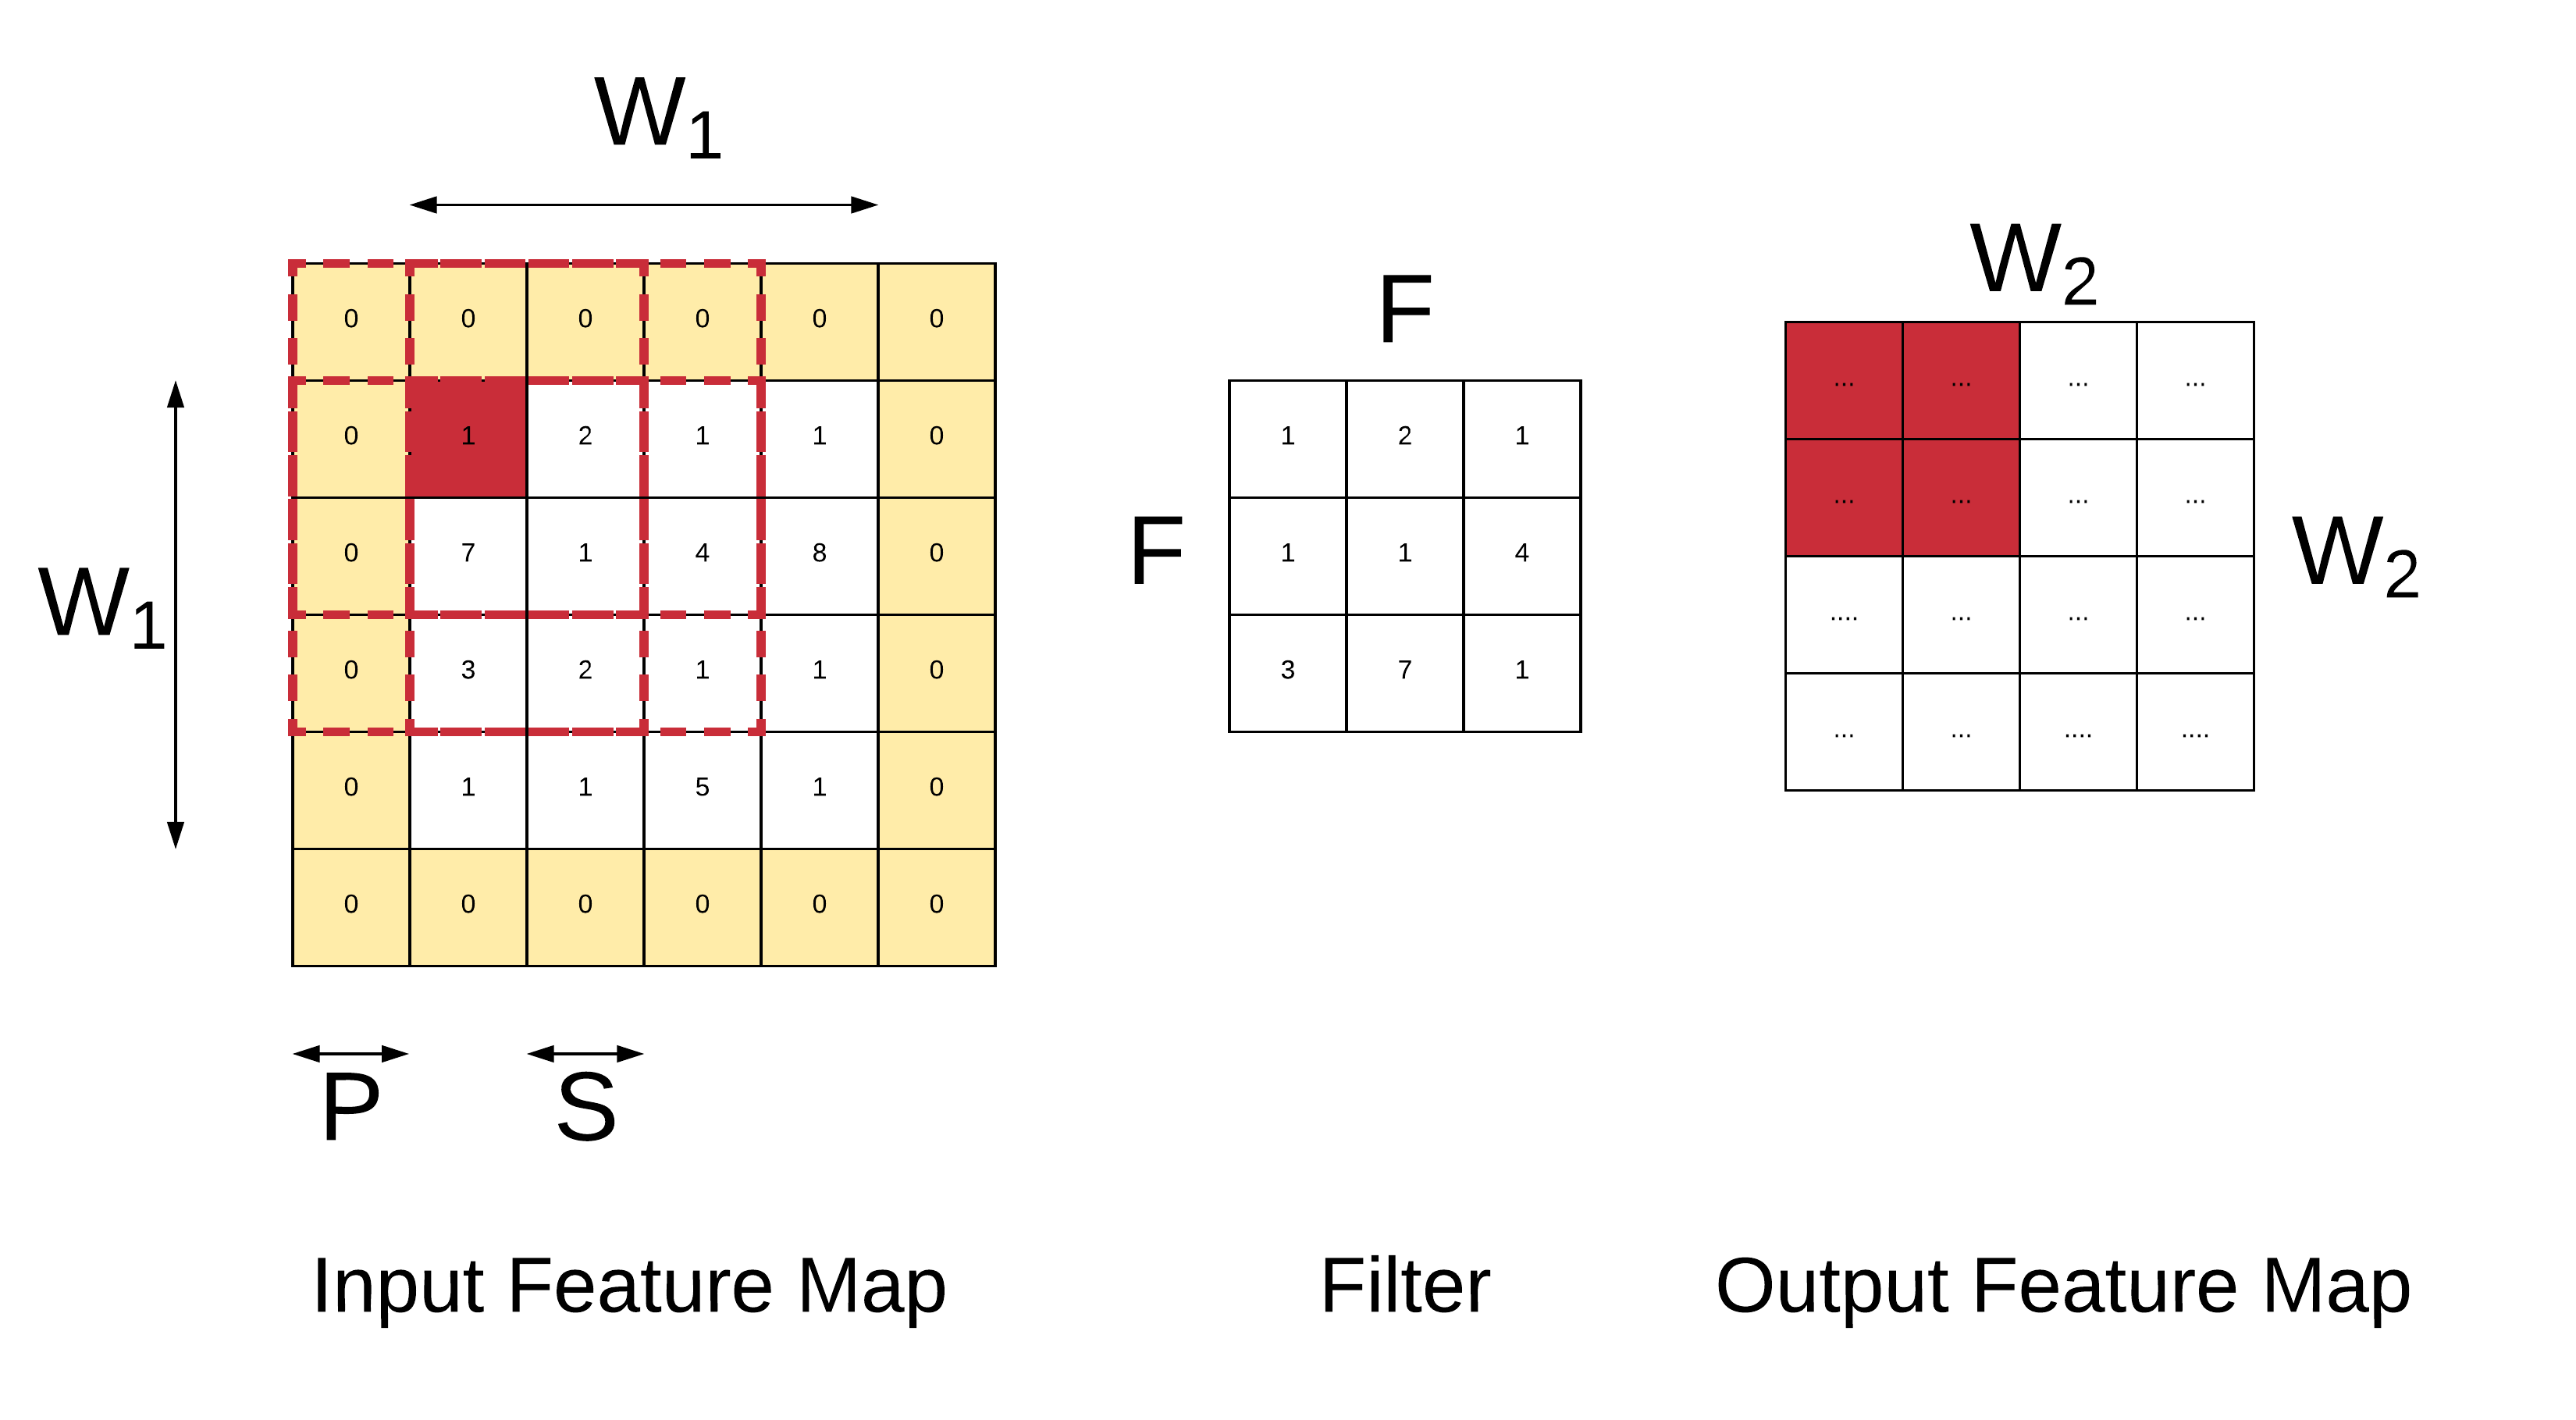
\includegraphics[width=\columnwidth]{./images/small_perturbations}
  \caption{Small perturbations in the input feature map only affect small regions in the output feature map after convolution}
  \label{fig:perturbation}
\end{figure}

More generally the propagation changes in the output feature map of a convolution or pooling layer caused by updating a patch in the input feature map is determined by the filter size $F$ and the stride $S$ of the Conv filter.
For example consider the situation shown in Figure. \ref{fig:patch_propagation}.
Assume a modified patch is placed on the input feature map which spans across $x_{in\_0}\rightarrow x_{in\_1}$ in $x$ dimension and $y_{in\_0}\rightarrow y_{in\_1}$ in y dimension.
Then the coordinates of the modified patch in the output feature map,  $x_{out\_0}\rightarrow x_{out\_1}$ in $x$ dimension and $y_{out\_0}\rightarrow y_{out\_1}$ in y dimension, can be expressed as a function of filter size $F$ and stride $S$ of the Conv/Pool filter as follows:

\begin{figure}
  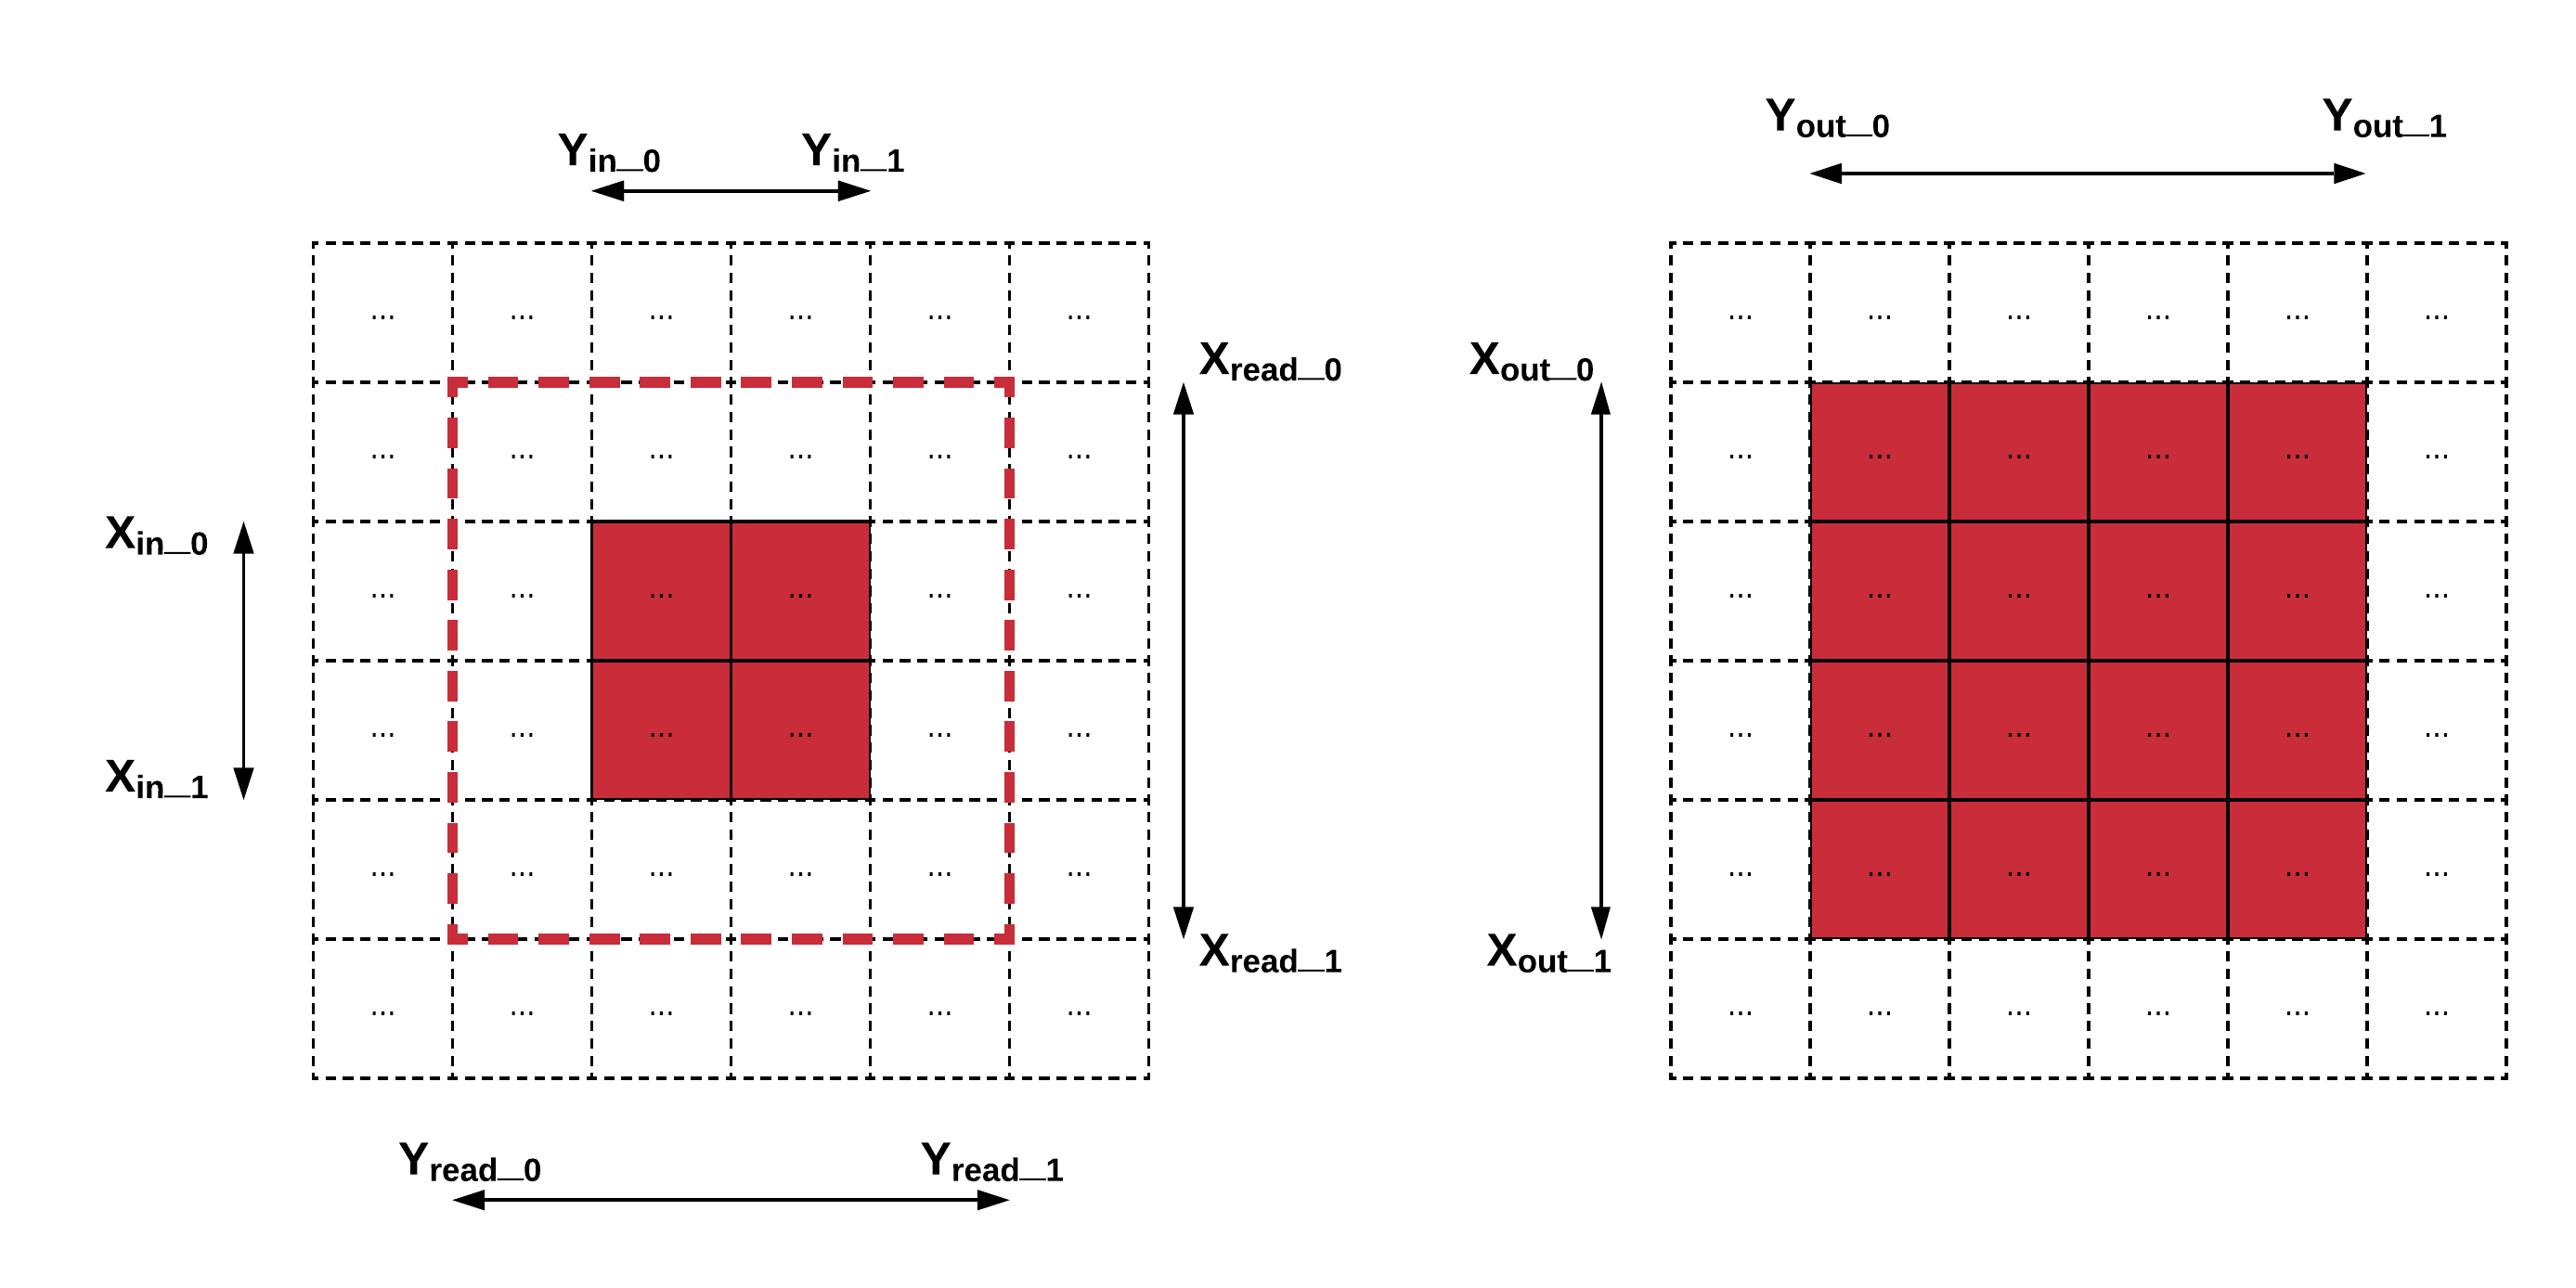
\includegraphics[width=\columnwidth]{./images/patch_propagation}
  \caption{Occlusion patch propagation in Conv layers}
  \label{fig:patch_propagation}
\end{figure}

\begin{equation}
x_{out\_0} = \texttt{max}(\texttt{ceil}((x_{in\_0} - F + 1)/S), 0) \\
\end{equation}
\begin{equation}
x_{out\_1} = \texttt{min}(\texttt{floor}((x_{in\_1} - 1)/S) + 1, W_2) \\
\end{equation}
\begin{equation}
y_{out\_0} = \texttt{max}(\texttt{ceil}((y_{in\_0} - F + 1)/S), 0) \\
\end{equation}
\begin{equation}
y_{out\_1} = \texttt{min}(\texttt{floor}((y_{in\_1} - 1)/S) + 1, W_2)\\
\end{equation}

\vspace{0.2in}

Also not that to compute these values in the output feature map we need to read a slightly bigger region from the input feature map due to the overlapping with the filter positions (marked in red dashed lines in Figure. \ref{fig:patch_propagation}). The coordinates of this read input patch, $x_{read\_0}\rightarrow x_{read\_1}$ in $x$ dimension and $y_{read\_0}\rightarrow y_{read\_1}$ in y dimension, is also a function filter size $F$ and stride $S$ of the Conv filter and can be expressed as follows:

\begin{equation}
x_{read\_0} = \texttt{max}(\texttt{ceil}((x_{in\_0} - F + 1)/S) \times S, 0) \\
\end{equation}
\begin{equation}
x_{read\_1} = \texttt{min}(\texttt{floor}((x_{in\_1} - 1)/S) \times S + F, W_1)\\
\end{equation}
\begin{equation}
y_{read\_0} = \texttt{max}(\texttt{ceil}((y_{in\_0} - F + 1)/S) \times S, 0) \\
\end{equation}
\begin{equation}
y_{read\_1} = \texttt{min}(\texttt{floor}((y_{in\_1} - 1)/S) \times S + F, W_2)\\
\end{equation}

\vspace{0.2in}

\begin{table}[t]
  \centering
  \caption{Notation used in Section. \ref{sec:ivm}}
  \scalebox{0.8}{\begin{tabular}{p{1cm}p{8.5cm}}
    \toprule
    \textbf{Symbol} & \textbf{Description}\\
    \midrule \midrule
    $W_1$ & Width of the input feature map to the Conv/Pool operator\\
    \midrule
    $D_1$ & Depth of the input feature map to the Conv operator\\
    \midrule
    $F$ & Width of filter kernel of the Conv/Pool operator\\
    \midrule
    $W_2$ & Width of the output feature map produced by the Conv/Pool operator\\
    \midrule
    $D_2$ & Depth of the output feature map produced by the Conv operator\\
    \midrule
    $x_{in\_0}$ & Starting x coordinate of the updated patch in the input feature map\\
    \midrule
    $x_{in\_1}$ & Ending x coordinate of the updated patch in the input feature map\\
    \midrule
    $y_{in\_0}$ & Starting y coordinate of the updated patch in the input feature map\\
    \midrule
    $y_{in\_1}$ & Ending y coordinate of the updated patch in the input feature map\\
    \midrule
    $x_{out\_0}$ & Starting x coordinate of the updated patch in the output feature map\\
    \midrule
    $x_{out\_1}$ & Ending x coordinate of the updated patch in the output feature map\\
    \midrule
    $y_{out\_0}$ & Starting y coordinate of the updated patch in the output feature map\\
    \midrule
    $y_{out\_1}$ & Ending y coordinate of the updated patch in the output feature map\\
    \midrule
    $x_{read\_0}$ & Starting x coordinate of the input feature map that need to be used for computing the updated output\\
    \midrule
    $x_{read\_1}$ & Ending x coordinate of the input feature map that need to be used for computing the updated output\\
    \midrule
    $y_{read\_0}$ & Starting y coordinate of the input feature map that need to be used for computing the updated output\\
    \midrule
    $y_{read\_1}$ & Ending y coordinate of the input feature map that need to be used for computing the updated output\\
    \bottomrule
  \end{tabular}}
\label{table:algo_symbols}
\vspace{-2mm}
\end{table}

\subsubsection{Estimating the maximum attainable theoretical speedup}

Important thing to notice with incremental inference of Conv and Pool layers for occlusion experiments is that the size of the updated patch in the output layer is larger than the updated patch in the input layer.
The growth is determined by the filter size and stride. Higher the filter size and stride higher the propagation rate of the modified patch.
With this observation, it is interesting to find out what percentage of computations can be saved by performing incremental inference of Conv and Pooling layers.
This can be easily estimated by iteratively calculating the updated patch sizes for Conv and Pooling layers based on the starting occlusion patch size $W_{patch}$ on the input image for all possible patch locations based on stride used $S_{patch}$.
Algorithm \ref{alg:max-speedup} shows how this can be calculated programmatically.
For sake of simplicity this algorithm assumes that the CNN architecture is a simple chained style architecture instead of more general style of directed-acyclic-graph (DAG).
However the algorithm can be easily extended support more general DAG style architectures.
It takes an object $CNN$ which is a nested information object containing information about different layers of the CNN and their properties, the size of the occlusion patch and the size of the stride for occlusion patch.
It then calculates the floating point operations required for incremental inference versus full inference for each possible location of the occlusion patch and computes the theoretical speedup which is the ratio between operation required for full inference and incremental inference.
It also computes the overall speedup which is the aggregation for all possible positions of the occlusion map and return this value along with 2D array containing individual position wise speedups as the output.

\begin{algorithm}
\caption{Estimate Maximum Theoretical Speedup}\label{alg:max-speedup}
\begin{algorithmic}[1]
\Procedure{EstimateMaxSpeedup}{$CNN$, $W_{patch}$, $S_{patch}$}
\State $flops_{inc} \gets 0$
\State $flops_{full} \gets 0$
\State $tmp \gets floor((CNN.image.W-W_{patch}+1)/S_{patch})$
\State $speedup \gets ARRAY[tmp][tmp]$

\For{\texttt{i in range(0, tmp, $S_{patch}$)}}
  \For{\texttt{i in range(0, tmp, $S_{patch}$)}}
      \State $tmp\_flops_{full} \gets 0$
      \State $tmp\_flops_{inc} \gets 0$
      
      \State $x_{in\_0} \gets i$
      \State $x_{in\_0} \gets i + W_{patch}$
      \State $y_{in\_0} \gets j$
      \State $y_{in\_0} \gets j + W_{patch}$

      \For{\texttt{k in range(0, size(CNN.layers), 1)}}
          \State $layer \gets CNN.layers[k]$
          \If {$layer.type$ $in$ $[conv, pool]$}
            \State $F \gets layer.filter.F$
            \State $S \gets layer.filter.S$
            
            \State $x_{out\_0} = \texttt{max}(\texttt{ceil}((x_{in\_0} - F + 1)/S), 0)$
            \State $x_{out\_1} = \texttt{min}(\texttt{floor}((x_{in\_1} - 1)/S) + 1, W_2)$
            \State $y_{out\_0} = \texttt{max}(\texttt{ceil}((y_{in\_0} - F + 1)/S), 0)$
            \State $y_{out\_1} = \texttt{min}(\texttt{floor}((y_{in\_1} - 1)/S) + 1, W_2)$

            \If {$layer.type$ $=$ $conv$}
              \State $W_1 \gets layer.input.W$
              \State $D_1 \gets layer.input.D$
              \State $W_2 \gets layer.output.W$
              \State $D_2 \gets layer.output.D$

              \State $tmp\_flops_{full} \mathrel{{+}{=}} F^2 \times D_1\times W_2^2\times D_2$
              \State $tmp\_flops_{inc} \mathrel{{+}{=}} F^2 \times D_1$
              \State $\hspace{10mm} \times ~(x_{out\_1} - x_{out\_0})$
              \State $\hspace{10mm} \times ~(y_{out\_1} - y_{out\_0})$
              \State $\hspace{10mm} \times ~D_2$
            \EndIf

            \State $(x_{in\_0}, x_{in\_1}, y_{in\_0}, y_{in\_1})$
            \State $\hspace{10mm} \gets (x_{out\_0}, x_{out\_1}, y_{out\_0}, y_{out\_1})$
          \ElsIf {$layer.type$ $=$ $fully-connected$}
            \State $W_1 \gets layer.input.W$
            \State $W_2 \gets layer.outputs.W$
            \State $tmp\_flops_{full} \mathrel{{+}{=}} W_1 \times W_2$
            \State $tmp\_flops_{inc} \mathrel{{+}{=}} W_1 \times W_2$
          \EndIf
      \EndFor

      \State $flops_{inc} \mathrel{{+}{=}} tmp\_flops_{inc}$
      \State $flops_{full} \mathrel{{+}{=}} tmp\_flops_{full}$
      \State $speedup[i][j] \gets tmp\_flops_{full}/tmp\_flops_{inc}$
      
  \EndFor
\EndFor

\State \textbf{return} ($flops_{full}$/$flops_{inc}$, $speedup$)
\EndProcedure
\end{algorithmic}
\end{algorithm}

We have applied this algorithm to analyze the theoretical maximum attainable speedup for many widely used CNN architectures by performing static analyzing on the CNN models defined using PyTorch framework (see Figure. \ref{fig:speedups}).
With an occlusion patch of size 16, moved with a stride of 1, for most CNN architectures we can achieve an average speedup of around 2.
However VGG and Squeezenet1\_0 CNN architectures can produce higher speedups than this.
The reason for this is VGG (16 and 19 layer versions) and Squeezenet1\_0 architectures use smaller Conv filter kernels $(3\times3)$. Therefore the rate of propagation of the occlusion patch is slower than other CNN architectures.
Thus more redundant computations can be saved from those architectures by applying incremental inference approach.

\begin{figure}
  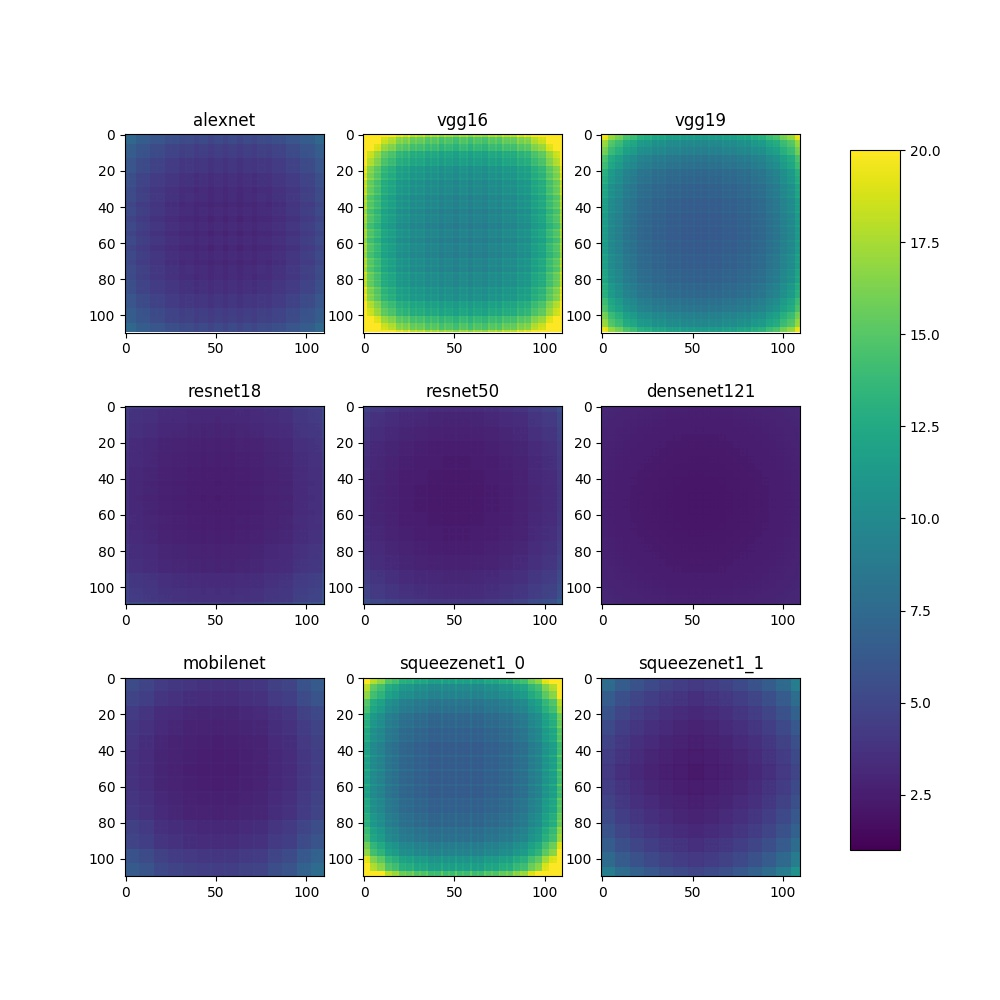
\includegraphics[width=\columnwidth]{./images/speedup_plots}
  \caption{Maximum attainable theoretical speedup for incremental inference approach for an occlusion experiment with patch of size 16 pixels stride of 2}
  \label{fig:speedups}
\end{figure}

\subsubsection{Occlusion Experiment with Incremental Inference}
With all the necessary core ideas explained, we now explain how incremental inference approach can be used to implement occlusion experiment (see Algorithm. \ref{alg:inc-inference}).
On a high-level the structure of this algorithm is similar to the theoretical speedup calculation algorithm. But the following differences can be noted. The algorithm takes an input image $I$ as input for the occlusion experiment in addition to the CNN model, patch width $W_{patch}$, and stride $S_{patch}$.
It then performs a full inference on the image and obtain a list containing activations for all the layers, including input image, by calling the method \texttt{PerformFullCNNInference(CNN, I)}.
It then finds the index of the predicted class label by finding the index of the maximum activation in the softmax layer, which is the last layer in the CNN.
Next similar to Algorithm. \ref{alg:max-speedup}, it iterates through all the possible positions of the occlusion patch on the input image and perform incremental inference for Conv and Pool layers based on the updated patch locations. For fully-connected and softmax layers usual full-inference is performed as there is no redundancy in computations.
When performing incremental inference for Conv and Pooling layers, the updated output of the previous layers is stitched together with pre-materialized values obtained from full inference ($M$) corresponding to that layer to create the input patch for the incremental inference operator.

Similar to speedup calculations, for simplicity, the algorithm here assumes the CNN architecture is a simple chain styled architecture. However it can be easily extended to support more general DAG style CNN architectures.
Another point to notice is that this algorithm performs inference for single occlusion position at a time. Alternatively one could batch together multiple occlusion patch positions together and perform batched inference. However since the patch sizes are not guaranteed to be the same at each layer, they may be need to be padded to transform them into the same size.
Batching multiple inferences together can reduce the runtime of occlusion experiments as it can amortize the overheads specially when using GPUs for inference.

\begin{algorithm}
\caption{Occlusion Experiment with Incremental Inference}\label{alg:inc-inference}
\begin{algorithmic}[1]
\Procedure{OcclusionWithIncrementalInference}{$I$,$CNN$, $W_{patch}$, $S_{patch}$}

\State $M \gets \texttt{PerformFullCNNInference}(CNN, I)$
\State $label_{index} \gets argmax(M[-1])$
\State $tmp \gets floor((CNN.image.W-W_{patch}+1)/S_{patch})$
\State $P \gets ARRAY[tmp][tmp]$

\For{\texttt{i in range(0, tmp, $S_{patch}$)}}
  \For{\texttt{i in range(0, tmp, $S_{patch}$)}}

      \State $x_{in\_0} \gets i$
      \State $x_{in\_0} \gets i + W_{patch}$
      \State $y_{in\_0} \gets j$
      \State $y_{in\_0} \gets j + W_{patch}$

      \State $x \gets Zero[x_{in\_1}-x_{in\_0}][y_{in\_1}][y_{in\_0}]$
      
      \For{\texttt{k in range(0, size(CNN.layers), 1)}}
          \State $layer \gets CNN.layers[k]$
          \If {$layer.type$ $in$ $[conv, pool]$}

            \State $x_{read\_0} \gets \texttt{max}(\texttt{ceil}((x_{in\_0} - F + 1)/S)$
            \State $\hspace{10mm} \times ~S, 0)$
            \State $x_{read\_1} \gets \texttt{min}(\texttt{floor}((x_{in\_1} - 1)/S)$
            \State $\hspace{10mm} \times ~S + F, W_1)$
            \State $y_{read\_0} \gets \texttt{max}(\texttt{ceil}((y_{in\_0} - F + 1)/S)$
            \State $\hspace{10mm} \times ~S, 0)$
            \State $y_{read\_1} \gets \texttt{min}(\texttt{floor}((y_{in\_1} - 1)/S)$
            \State $\hspace{10mm} \times ~S + F, W_2)$

            \State $tmp \gets M[k]$
            \State $tmp[x_{in\_0}:x_{in\_1}][y_{in\_0}:y_{in\_1}] \gets x$

            \State $x \gets tmp[x_{read\_1}-x_{read\_0}]$
            \State $\hspace{20mm}       [y_{read\_1}-y_{read\_0}]$

            \State $x \gets layer.transform(x)$

            \State $F \gets layer.filter.F$
            \State $S \gets layer.filter.S$
            
            \State $x_{out\_0} = \texttt{max}(\texttt{ceil}((x_{in\_0} - F + 1)/S), 0)$
            \State $x_{out\_1} = \texttt{min}(\texttt{floor}((x_{in\_1} - 1)/S) + 1, W_2)$
            \State $y_{out\_0} = \texttt{max}(\texttt{ceil}((y_{in\_0} - F + 1)/S), 0)$
            \State $y_{out\_1} = \texttt{min}(\texttt{floor}((y_{in\_1} - 1)/S) + 1, W_2)$
            
            \State $(x_{in\_0}, x_{in\_1}, y_{in\_0}, y_{in\_1})$
            \State $\hspace{10mm} \gets (x_{out\_0}, x_{out\_1}, y_{out\_0}, y_{out\_1})$
          \ElsIf {$layer.type$ $=$ $fully-connected$}
            \State $tmp \gets CNN.layers[k-1].type$
            \If {$tmp \mathrel{{!}{=}} fully-connected$}
              \State $tmp \gets M[k-1]$
              \State $tmp[x_{out\_0}:x_{out\_1}]$$[y_{out\_0}:y_{out\_1}]$$\gets x$
              \State $x \gets tmp$
            \EndIf
            \State $x \gets fully-connected(x, layer.weights)$
          \ElsIf {$layer.type$ $=$ $softmax$}
            \State $x \gets softmax(x)$
          \EndIf
      \EndFor

      \State $P[i][j] \gets x[label_{index}]$
      
  \EndFor
\EndFor

\State \textbf{return} $(label_{index}, P)$
\EndProcedure
\end{algorithmic}
\end{algorithm}

\section{Early Experimental Results}
In this section we summarize the early experimental results obtained by implementing the incremental inference for occlusion experiments.

\textbf{Experimental Setup.} The experiments was performed on an Intel(R) Core(TM) i7-6700 CPU 3.40GHz machine with 32 GB RAM. The machine is also equipped with a Nvidia Titan Xp GPU. We use PyTorch 0.3.1 library as the deep learning toolkit library.

\textbf{Workload}. We use a popular ImageNet pre-trained VGG 16 layer CNN model and subject it to occlusion experiments. The performance of the occlusion experiment with naive approach and incremental inference approach is benchmarked on CPU and GPU separately.
An occlusion patch of size $16\times16$ was placed on the center of the image of size $224\times224$ and runtime for full inference approach and incremental inference approach average over 5 iterations is recorded. From these values the speedup is calculated. The experiment was repeated with a batch size of 1 and 16 (see Table. \ref{table:speedup}).

\begin{table}[h]
\centering
\begin{tabular}{|l|l|l|l|}
\hline
\multirow{2}{*}{Batch Size} & \multirow{2}{*}{Theoretical Speedup} & \multicolumn{2}{l|}{Experimental Speedup} \\ \cline{3-4} 
 &  & CPU & GPU \\ \hline
1 & 7.6 & 5.4 & 1.3 \\ \hline
16 & 7.6 & 5.4 & 1.6 \\ \hline
\end{tabular}
\caption{Theoretical versus empirical speedup achievable with incremental inference}
\label{table:speedup}
\end{table}
\vspace{-5.mm}

Our implementation of incremental inference of Conv and Pool layers could achieve a speedup of 5.4 on CPU for a batch size of 1 and 16 compared to the theoretical maximum speedup of $7.4$. However, the GPU implementation could achieve a speedup of only 1.3 and this can be increased upto 1.6 with a batch size of 16. We suspect that the random memory operations introduced by the incremental inference approach due to stitching of output of incremental Conv and Pool layers with pre-materialized activations of the full inference is  throttling the GPU performance in incremental approach.

\section{Conclusions \& Future Work}
In this work explore applying incremental inference of Conv and Pooling layers of CNN models to reduce the runtime of occlusion experiments.
We formalize the incremental inference approach for CNNs and evaluate the theoretical upper-bound of speedup achievable for different CNN architectures by statically analyzing the CNN architecture definitions specified in PyTorch framework.
For most CNN architectures we can achieve a speedup higher than 2 and for some CNN architectures, such as VGG and Squezenet1\_0, this can be higher than $7$.
Our implementation of incremental inference of Conv and Pool layers could achieve a empirical speedup of 5.4 on CPU and 1.6 on GPU with a batch size of 16. We suspect the relatively low speedup of GPU implementation is attributable to the random memory operations caused by incremental inference throttling the GPU performance.

As future work we are looking in to developing a more efficient GPU implementation which can attain higher speedup. This will require implementing GPU kernels which can perform incremental Conv and Pooling operations in place without additional memory copying.
We also plan to explore several other optimizations including explore and exploit style approaches on localizing the most sensitive image regions and approximate CNN inference for reducing the runtime of occlusion based CNN explainability workloads.
Explore and exploit style approach is an algorithmic optimization motivated by the specific use cases of occlusion experiments.
In most applications such as medical imaging the objects of interest in an image occupies a relatively small portion and are located together.
In such settings rather using a patch of small size we can start with a large patch with a relatively large stride and then iteratively focus into smaller regions which appears to be sensitive for the predicted class label.
% We name this approach as \textit{hierarchical inference of occlusion patches}.
Approximate inference of CNN approach is based on a general observation of deep CNN inference.
Even though in theory the projective field of an input pixel grows linearly in practice the effective projective field does not grow in that rate.
This mean most of the local changes in the input space are affecting localized changes in the output space of a convolution operation.
Therefore we plan to experiment the possibility of constraining the growth of the projective field of an input pixel and there by reduce runtime using our \textit{incremental inference} approach.
% We name this optimization as \textit{approximate inference} of deep CNNs.

\bibliographystyle{abbrv}
\bibliography{main}
\end{document}